
\section{Motivation}
\label{sec:motivation}



\subsection{An example of a commit }
\label{sec:examle}

\begin{figure*}
\center
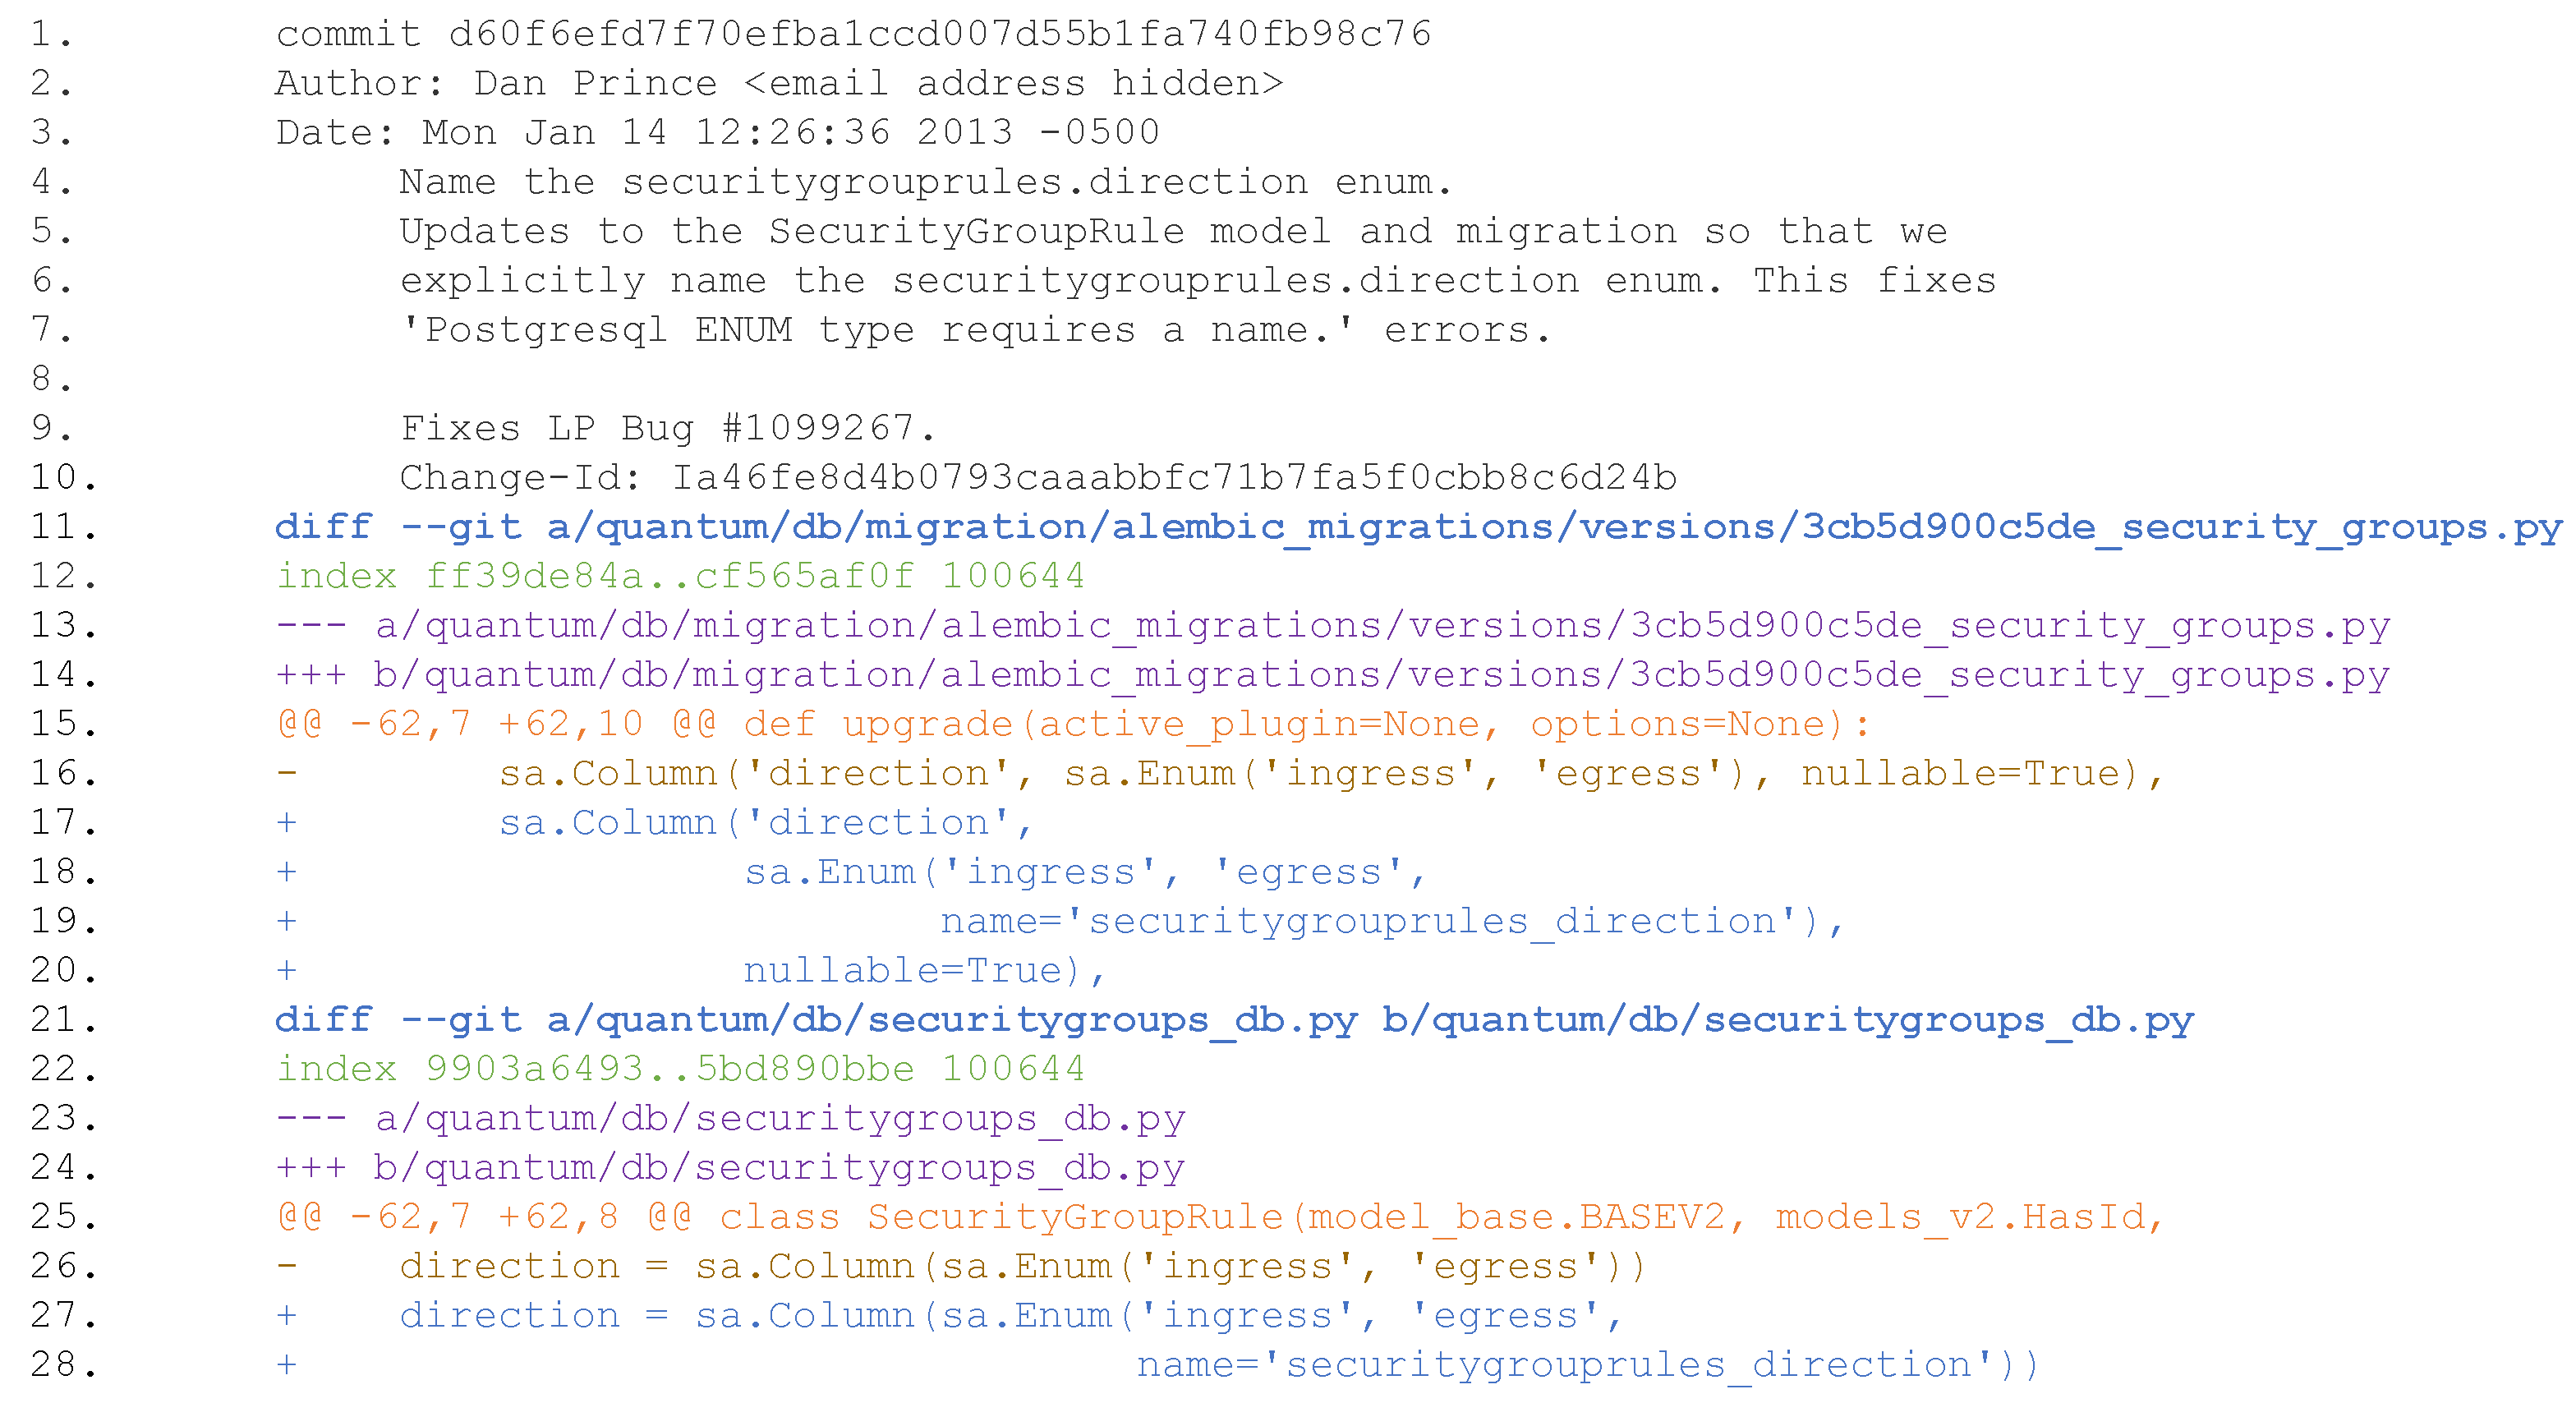
\includegraphics[scale=0.3]{figs/example.pdf}
\caption{An example of a commit change.}
\label{fig:example}
\end{figure*}


\subsection{Convolutional Neural Networks}
\label{sec:background_cnn}

\begin{figure*}[t!]
	\center
	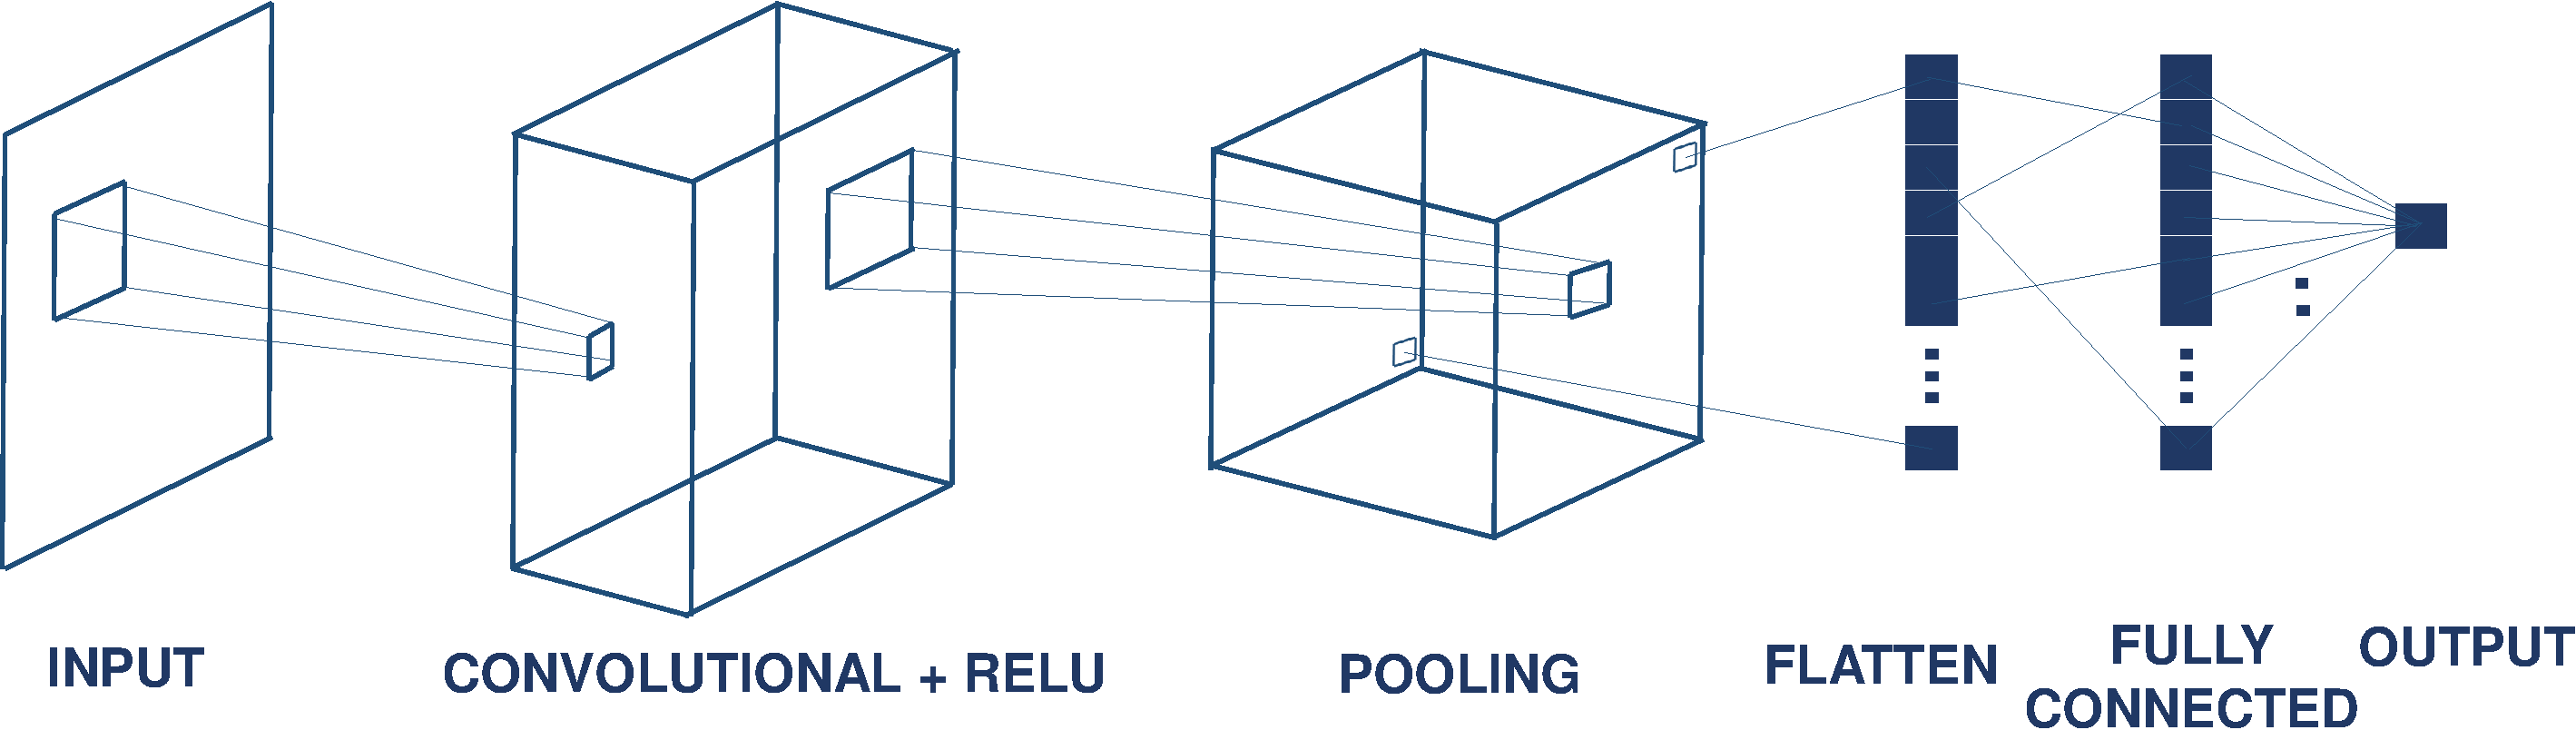
\includegraphics[scale=0.3]{figs/cnn.pdf}
	\caption{A simple convolutional neural network architecture.}
	\label{fig:cnn}
\end{figure*}

\begin{figure*}[t!]
	\center
	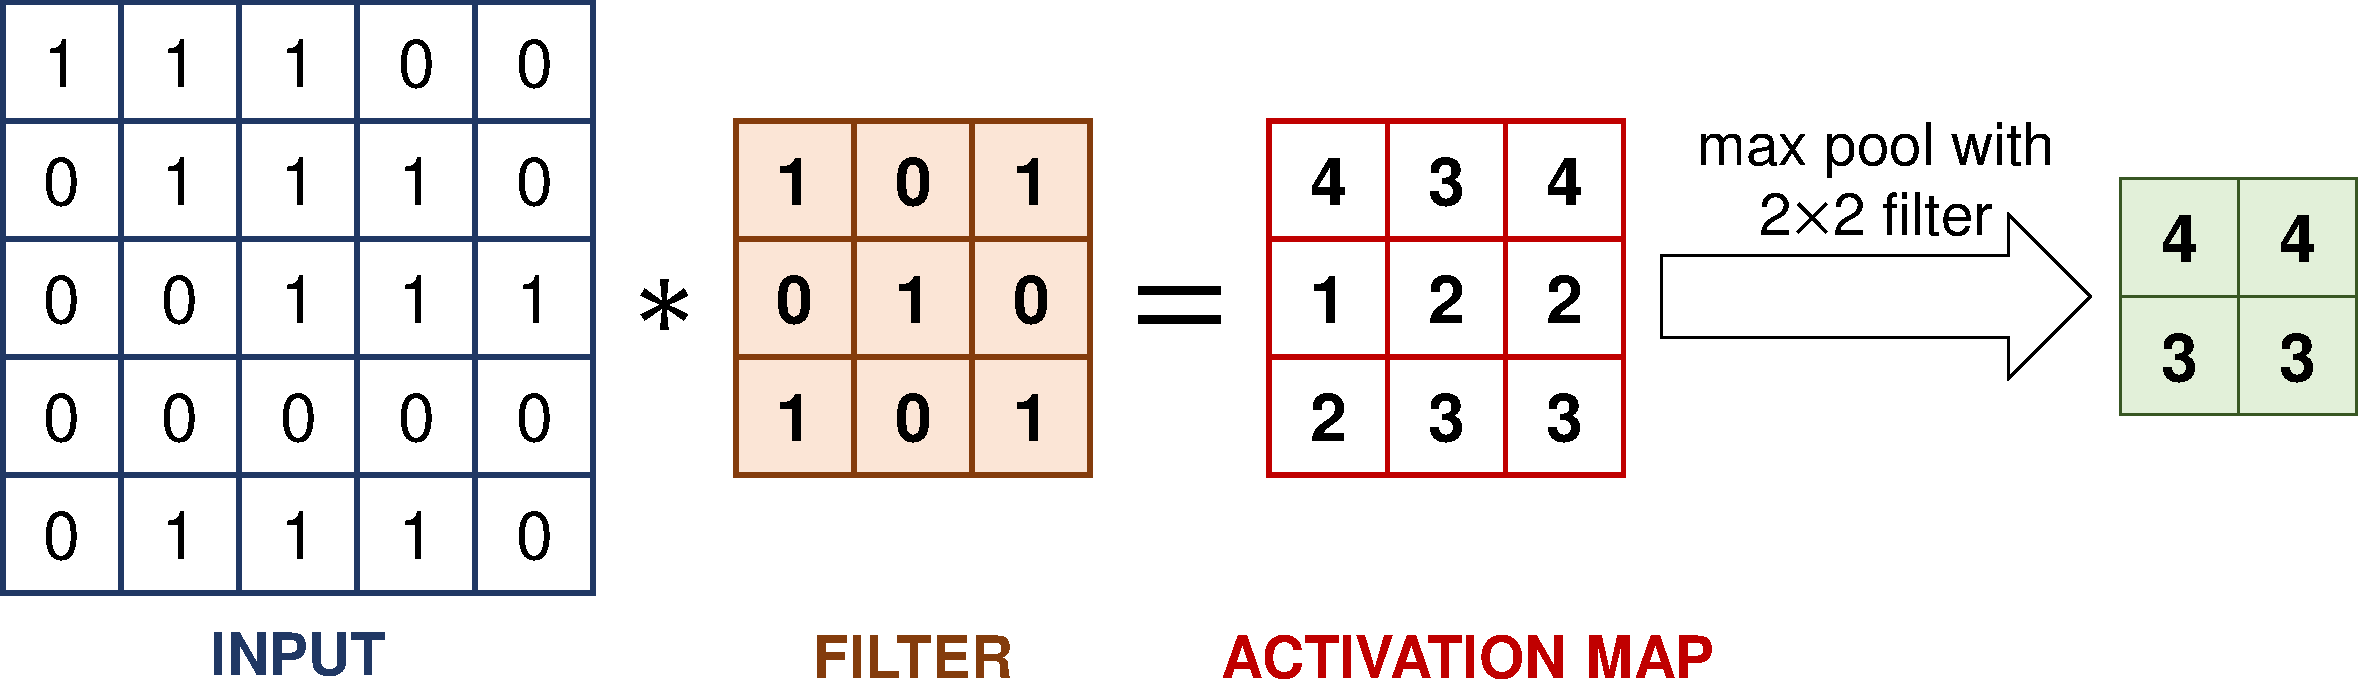
\includegraphics[scale=0.3]{figs/filter_pooling.pdf}
	\caption{An example of a convolutional layer and pooling layer in CNN.}
	\label{fig:filter}
\end{figure*}

One of the most powerful forms of deep learning neural networks is the Convolutional Neural Network (CNN)~\cite{lecun2015deep}. CNNs are widely used to solve image pattern recognition problems and have been achieved significant results~\cite{karpathy2014large, lawrence1997face, krizhevsky2012imagenet}. Like traditional deep learning networks, CNNs receive an input and perform a product operation followed by a nonlinear function. The last layer is the output layer containing objective functions~\cite{zhao2017loss} associated with the labels of the input.

Figure~\ref{fig:cnn} illustrates a simple CNN for classification task. The simple CNN includes an input layer, a convolutional layer, followed by the rectified linear unit (RELU) which is a nonlinear activation function, a pooling layer, a fully-connected layer, and an output layer. We briefly explain these layers in the following paragraphs. 

The input layer takes an input as 2-dimensional array or 3-dimensional array and passes it through a of convolution layers.

The convolutional layer plays a vital role in CNN and it takes advantage of the use of learnable filters. These filters are small in spatial dimensionality, but they are applied along the entirety of the depth of the input data. For example, given an input data $\textbf{I} \in \mathbb{R}^{\text{H} \times \text{W} \times \text{D}}$ and a filter $\textbf{K} \in \mathbb{R}^{\text{h} \times \text{w} \times \text{D}}$, we produce a new activation map $\textbf{A} \in \mathbb{R}^{(\text{H} - \text{h}) \times (\text{W} - \text{w}) \times 1}$. The RELU is then applied to each value of the activation map as follows:
\begin{equation}
\label{eq:relu}
f(x) = max(0, x)   
\end{equation}

The pooling layer, which is an important component of CNN, aims to reduce the dimensionality of the activation map, the number of parameters, and the computational helping to control overfitting problem~\cite{tolias2015particular}. The pooling layer spreads along the activation map and scales its dimensionality. There are three different types of pooling layers:
\begin{itemize}
	\item Max pooling takes the largest element from each region of the activation map.
	\item Average pooling constructs the average value from each region of the activation map.
	\item Sum pooling sums all the elements from each region of the activation map. 
\end{itemize}
In practice, max pooling often achieves a better performance compared to the other two pooling techniques~\cite{zeiler2013stochastic}. Figure~\ref{fig:filter} presents a visual representation of a convolutional layer and pooling layer in CNN. Given an input 5$\times$5 and a filter 3$\times$3, we output a new activation map 3$\times$3. A max pooling layer with a filter 2$\times$2 is then applied to produce a new output. 

The output of pooling layer is flatten and directly passed to a fully connected layer (or a hidden layer). The fully connected layer is passed to an output layer to calculate an objective function (or a loss function)~\cite{zhao2017loss}. The objective function normally is optimized using a stochastic gradient descent (SGD)~\cite{bottou2010large}. This is an analogous way with traditional neural networks~\cite{huang1988neural}.



